\section{Theoretical Framework and Mathematical Formulation}
\label{sec:matform}

Auxiliary-field, or Determinant \acs{QMC} is a simulation method that is commonly used to simulate the Hubbard model, allowing one to capture the elusive effects of electron correlations in the two-dimensional graphene-like nanostructures we are concerned with.
The sign problem may deem the algorithm exponentially complex in the size of the system and in inverse temperature, but it is possible to overcome this hurdle for a class of models, namely the Hubbard model on a bipartite lattice at half filling ($\mu = 0$ in our conventions).
In fact, many interesting phenomena occur at half filling, for example magnetic ordering and the Mott metal-insulator transition.
The difficulty lies in computing the nearly vanishing average of a random variable $X$ with comparatively large variance, i.e. $\sigma_X / \left\langle X \right\rangle \gg 1$.

Ultimately, we seek a computable approximation of the projection operator $\mathcal{P}$ defined in equation (\ref{eq:projection}).
As we shall see, it is found by using (either a discrete or continuous) Hubbard-Stratonovich transformation.
This transformation introduces an auxiliary field (consisting basically of Ising spins), and we use Monte Carlo to sample configurations from the distribution corresponding to this \emph{classical} configuration space.
This approach is equivalent to an exact solution of the integral that is approximated by using the saddle point approximation in mean field, an observation which motivates us to compare our results with the mean field ones.
Mean field theory may be formulated by applying the Hubbard Stratonovich (HS)  transformation to transform an interacting problem into a one-body problem, and then apply the saddle-point approximation to solve the resulting integrals.
In the \acs{GCE} (where we make $\mathcal{H} \mapsto \mathcal{H} - \mu \mathcal{N}$, $\mathcal{N}$ being the total particle number), the partition function may be written in terms of a functional integral over a space-time dependent field of the exponential of a one-body action
\begin{equation}
Z = \Tr [ e^{-\beta \mathcal{H} } ] = \int \mathcal{D}\bm h \, e^{-S(\bm h) }  \equiv \Tr_{\bm h} [ e^{-S(\bm h)} ],
\end{equation}
which may be computed by Monte Carlo sampling.
In mean field, we approximate the integral by replacing the functional integral by a constant times the exponential action itself evaluated at a single field $\bm h^\star$, for which the action has a minimum: $\partial_{\bm h} S( \bm h ) |_{\bm h = \bm h^\star} = 0$, and $\partial_{\bm h}^2 S( \bm h ) |_{\bm h = \bm h^\star} > 0$.

The integral is evaluated exactly in the auxiliary field \acs{QMC} method, which avoids the bias introduced by the specific choice of the HS decoupling.
The nature of the analytical mean field solution depends on this choice, while the unbiased \acs{QMC} solution does not, relying on a numerical solution that scales with the cubic volume of the system, and linearly with inverse temperature.

The sign problem may be seen as an inherent difficulty that arises from taking all possible fluctuations around the mean field solution.
An advantage of determinant \acs{QMC} is that certain symmetries of the model at hand, such as \acs{PHS} in the Hubbard model, may be used to avoid the sign problem.

\subsection{Trotter-Suzuki Decomposition}
\label{subsec:trotter}

In section \ref{sec:exactSolutions}, we found exact solutions for particular instances of the Hubbard model by finding a closed form for the partition function \cite{hou_numerical_2009}. When devising a numerical method, a good sanity check is to verify that it satisfactorily approximates the partition function since it is the quantity that can be used to obtain  any observable.
Computing the partition function of a quantum system in equilibrium
\begin{equation}\label{eq:partitionBeta}
Z_\beta = \text{Tr} \big[ e^{-\beta \mathcal{H} } \big] = \sum_{\alpha} \left\langle \psi_\alpha | e^{-\beta \mathcal{H} } | \psi_\alpha \right\rangle
\end{equation}
is equivalent to studying its \emph{imaginary} time evolution.
The inverse temperature $\beta$ represents the imaginary time $\tau = it$, and $Z_\beta$ may be simply thought of as the wave function of the analogous quantum system at imaginary time $\beta$.
%To see this, recall that quantum states evolve according to
%
%\begin{equation}
%\left| \psi (t) \right\rangle = e^{-i \mathcal{H} t } \left| \psi (0) \right\rangle \iff \left| \psi (\tau) \right\rangle = e^{-\tau \mathcal{H} } \left| \psi (0) \right\rangle,
%\end{equation}
%
%Taking the scalar product with a position eigenstate $ \left\langle \bm x \right|$, we obtain $\psi (\bm x, \beta) = \left\langle \bm x | \psi (\beta) \right\rangle$.
%Using the closure relation $\int d\bm y \left| \bm y \right\rangle  \left\langle \bm y \right| = 1$, we get
%
%\begin{equation}
%\psi ( \bm x , \tau ) = \int d\bm y \left\langle \bm x | e^{-\tau \mathcal{H}} | \bm y \right\rangle \psi (\bm y, 0)
%\end{equation}
%
%The wave function at position $\bm x$ and time $\tau$ may be obtained by this equation as long as we know the wave function at $\tau = 0$, $\psi (\bm y, 0)$ for all points in space $\bm y$. The Green's function
%
%\begin{equation}
%G ( \bm x, \tau | \bm y, 0 ) \equiv \left\langle \bm x | e^{-\tau \mathcal{H}} | \bm y \right\rangle ,
%\end{equation}
%satisfies the Schr\"odinger equation, subject to the initial condition $\psi (\bm y, 0) = \delta (\bm y - \bm x )$. Thus, it corresponds to the probability of presence at $\bm x, \tau$ of a wave packet centered at $\bm y$ at $\tau = 0$. Thus, solving the Schr\"odinger equation is  analogous to solving the diffusion equation (that in turn one may obtain as the continuum limit of a random walk). We may write $G$ as a linear combination of the eigenstates of the Hamiltonian
%
%\begin{equation}
%G (\bm x, \tau | \bm y, 0) = \sum_\alpha \psi_\alpha^\star (\bm y) \psi_\alpha (\bm x) e^{-E_\alpha \tau}  ,
%\end{equation}
%so that
%
%\begin{equation}\label{eq:psiZ}
%\psi ( \bm x, \tau ) = \sum_\alpha \int d\bm y \, \psi_\alpha^\star (\bm y) \psi_\alpha (\bm x) e^{-E_\alpha \tau} \delta ( \bm y - \bm x ) = \sum_\alpha \psi_\alpha^\star (\bm x) \psi_\alpha (\bm x) e^{-E_\alpha \tau} = \sum_{\alpha} \left\langle \psi_\alpha | e^{-\tau \mathcal{H} } | \psi_\alpha \right\rangle
%\end{equation}
%where we immediately notice a striking similarity with equation (\ref{eq:z_asEigen}), by making $\psi (\bm x, \tau) \mapsto Z_\beta$.
In fact, for a zero temperature system, projective methods use this same principle to find the ground state.
In that case, the partition function strictly corresponds to the ground state wave function when $\tau \rightarrow \infty$ (in practice, one takes $\tau = \Theta$ large enough).
%As we can see from Eq.(\ref{eq:psiZ}), the higher energy states are exponentially suppressed in this limit, so that $\psi (\bm x, \tau) \rightarrow |\psi_0 (x)|^2 e^{-E_0 \tau}$.
%The initial condition does not even have to be $\psi ( \bm y, 0) = \delta ( \bm y - \bm x )$.
%More generally, as we saw for diffusion \acs{QMC}, we only require $\int d\bm y \, \psi_0^\star ( \bm y ) \psi ( \bm y, 0 ) = C \neq 0$, and we obtain $\psi (\bm x, \tau\rightarrow \infty) \rightarrow C \psi_0 (x) e^{-E_0 \tau}$.
 
Eq.(\ref{eq:partitionBeta}) is not very amenable to numerical computation since it contains an exponential of a sum of non-commuting operators $e^{-\beta (\mathcal{H}_K + \mathcal{H}_V)}$ as per Eq.(\ref{eq:def_energies}). 
The exponential is not factorizable and involves computing an infinite number of commutators containing these two operators, as per the Zassenhaus formula, valid for any two generic operators $X$ and $Y$\footnote{This is just the inverse of the well known Baker–Campbell–Hausdorff formula commonly used in quantum mechanics.}:
\begin{equation}\label{eq:zassenhaus}
e^{\delta (X+Y)}=e^{\delta X} e^{\delta Y} e^{-{\frac {\delta^{2}}{2}}[X,Y]} e^{{\frac {\delta^{3}}{6}}(2[Y,[X,Y]]+[X,[X,Y]])}  e^{{\frac {-\delta^{4}}{24}}([[[X,Y],X],X]+3[[[X,Y],X],Y]+3[[[X,Y],Y],Y])} \, ... , 
\end{equation}
where $\delta \in \mathbb{C}$ is an expansion parameter.
The Trotter-Suzuki decomposition leads to the sought approximate factorization that is used to approximate the partition function.
Dividing the imaginary time interval $[0, \beta ]$ into $L$ equal sub-intervals of small width $\Delta \tau = \beta / L$:
\begin{equation}\label{eq:partBreak}
Z =  \Tr \bigg[ \prod_{l=0}^{L-1} e^{-\Delta\tau \mathcal{H} } \bigg] ,
\end{equation}
we obtain a form that is more amenable to computation.
Actually, it also arises naturally by writing the matrix elements of the projection operator $\mathcal{P}$ as path integrals (here, time ordering is implicit \cite{hirsch_discrete_1983}):
\begin{equation}
\left\langle \psi | e^{-\beta \mathcal{H} } | \psi' \right\rangle = \sum_{\left| \psi_1 \right\rangle, \left| \psi_2 \right\rangle,..., \left| \psi_{L-1} \right\rangle }  \left\langle \psi | e^{-\Delta \tau \mathcal{H} } | \psi_1 \right\rangle \left\langle \psi_1 | e^{-\Delta \tau \mathcal{H} } | \psi_2 \right\rangle ... \left\langle \psi_{L - 1} | e^{-\Delta \tau \mathcal{H} } | \psi' \right\rangle 
\end{equation}

Then, the partition function only selects paths that are periodic in imaginary time:
\begin{equation}
Z = \text{Tr} \big[ e^{-\beta \mathcal{H} } \big] = \sum_{\left| \psi_0 \right\rangle} \left\langle \psi_0 | e^{-\beta \mathcal{H}} | \psi_0 \right\rangle = \sum_{\{ \left| \psi_l \right\rangle \}} \prod_{l = 0}^{L - 1} \left\langle \psi_{l} | e^{-\Delta \tau \mathcal{H} } | \psi_{l+1} \right\rangle \delta_{0, L} = \Tr \bigg[ \prod_{l=0}^{L-1} e^{-\Delta\tau \mathcal{H} } \bigg] ,
\end{equation}
where we have $\left| \psi_L \right\rangle = \left| \psi_0 \right\rangle$, and we  recover the result of Eq.(\ref{eq:partBreak}) by simply reorganizing the summations over $\{ \left| \psi_l \right\rangle \}$, so as to make appear closure relations, resulting in unit operators in the Hilbert space of each slice.
The \say{Trotter breakup} follows from truncating Eq.(\ref{eq:zassenhaus}), and keeping only the first order term in $\Delta \tau$.
In the $\Delta \tau \rightarrow 0$ limit, it becomes a trace of a time ordered exponential of the integral of the time-dependent action.
The slice index $l$, or the argument $\tau$, imply time ordering.
\begin{equation}\label{eq:Z_propagator}
Z = \Tr \bigg[ \prod_{l=0}^{L-1} e^{-\Delta\tau \mathcal{H}_{K}^l } e^{-\Delta\tau \mathcal{H}_{V}^l } \bigg] + \mathcal{O}(\Delta \tau^2) \underset{\tau \rightarrow 0}{\longrightarrow}
 \Tr \bigg[ \mathcal{T}_\tau \exp \bigg( {- \int_0^\beta   d\tau ( \underbrace{\mathcal{H}_K (\tau) + \mathcal{H}_V ( \tau) ) }_{S(\tau)} } \bigg) \bigg]
\end{equation}

\subsection{Hubbard-Stratonovich transformation}\label{subsec:HStransf}

The kinetic energy term is quadratic in the fermion operators, and is spin-independent and thus may be separated into spin up and spin down components, independent of the time slice, i.e. $\mathcal{H}_{K_\sigma}^l = \mathcal{H}_{K_\sigma}$.
\begin{equation}
e^{-\Delta\tau \mathcal{H}_K} = e^{-\Delta\tau \mathcal{H}_{K_\uparrow}} e^{-\Delta\tau \mathcal{H}_{K_\downarrow}} ,
\end{equation}
where $\mathcal{H}_{K_\sigma} = \bm c_\sigma^\dagger (-t_\sigma \bm K_\sigma - \mu_\sigma \bm I )  \bm c_\sigma$, and we allow spin-dependent hoppings and chemical potential.

The potential energy term, however, is quartic.
Fortunately, it is possible to express it in quadratic form by introducing an extra degree of freedom, the so called \emph{Hubbard-Stratonovich (HS) field} $\bm h \equiv (h_{l, i})_{i=0,\, l= 0}^{N-1, \, L - 1}$, in which each element is essentially an Ising spin.
At each slice, the interaction is eliminated by an $N$-dimensional HS field $\widetilde{\bm h}$.
We start by noting that $[ n_i , n_j ] = 0 \,\, \forall i, j$, so that
\begin{equation}\label{eq:Hint}
e^{-\Delta\tau \mathcal{H}_V} = e^{-U \Delta\tau \sum_{i=1}^N (n_{i\uparrow} - 1/2 ) (n_{i\downarrow} - 1/2 )} = \prod_i e^{-U \Delta\tau (n_{i\uparrow} - 1/2 ) (n_{i\downarrow} - 1/2 )}
\end{equation}

The HS transformation is based on the well known identity 
$
e^{ \frac{a^2}{2}} = \frac{1}{\sqrt{2\pi}} \int_{-\infty}^{\infty} e^{-\frac{z^2}{2}  - za } dz
$ 
$ \forall a > 0$, 
which is also valid for an operator $\mathcal{A}$, that is, making $a \mapsto \mathcal{A}$ in the Gaussian integral identity.
Noting that $(n_{i\uparrow} - \frac{1}{2} ) (n_{i\downarrow} - \frac{1}{2} ) = -\frac{1}{2} ( n_{i\uparrow} - n_{i\downarrow} )^2 + \frac{1}{4}$, we can recast the potential energy term as
\begin{equation}
e^{-\Delta\tau \mathcal{H}_V} = \prod_i e^{ \frac{U \Delta \tau}{2} ( n_{i\uparrow} - n_{i\downarrow} )^2 } e^{- \frac{U \Delta \tau}{4}}
=\bigg( \frac{\Delta \tau e^{- \frac{U \Delta \tau}{2}}}{\pi} \bigg)^{N/2} \int_{-\infty}^\infty \prod_i d \widetilde{h}_i e^{-\Delta \tau [ \widetilde{h}_i^2 + \sqrt{2U} ( n_{i\uparrow} - n_{i\downarrow} ) \widetilde{h}_i ]} ,
\end{equation}
so that in the $\tau \rightarrow 0$ limit, the partition function becomes
\begin{equation}
Z \propto \int \mathcal{D} \widetilde{\bm h} ( \tau) e^{-\int_0^\beta d\tau \widetilde{\bm h}^2 ( \tau ) } \Tr \bigg[ \mathcal{T}_\tau e^{ -\int_0^\beta d\tau [ \mathcal{H}_K ( \tau ) + \sqrt{2U} ( \bm n_{\uparrow} (\tau) - \bm n_{\downarrow} (\tau ) ) \cdot \widetilde{\bm h}(\tau) ] } \bigg] ,
\end{equation}
representing a system of noninteracting fermions coupled via spin $s^z$ to an external fluctuating real field.

The fact that $n_{i,\sigma}$ can only take on two possible values suggests an analogous transformation in which the fluctuating field can only take on two possible values.
An Ising spin will prove sufficient to eliminate the direct electron-electron interaction.
The discrete HS transformation for $U > 0$ allows us to recast Eq.(\ref{eq:Hint}) in terms of the local spin, a non-interacting quadratic term $n_{i\uparrow} - n_{i\downarrow} $ (at each imaginary-time slice, since the operators live on the Hilbert space of that specific slice).
Let $c_U = \frac{1}{2} e^{-\frac{U\Delta \tau}{4}}$ and $\nu = \text{arcosh} ( e^{\frac{U\Delta\tau}{2}})$.
Then, the sought transformation reads
\begin{equation}\label{eq:discreteHS}
e^{-U \Delta\tau (n_{i\uparrow} - 1/2 ) (n_{i\downarrow} - 1/2 )} = c_U \sum_{\widetilde{h}_i = \pm 1} e^{\nu \widetilde{h}_i (n_{i\uparrow} - n_{i\downarrow} )}
\end{equation}

Notice that $\Delta \tau$ appears explicitly in the coupling constant.
This is because we worked with fixed length Ising spins.
In the Gaussian formulation we started with, $\Delta \tau$ can be reabsorbed in the HS field, even though $\Delta \tau$ is still implicit in the integration measure.
The parameter $\frac{1}{\Delta \tau}$ can be seen as a high energy cutoff, and it must be larger than all other energy scales in the problem, which is required to make the Trotter breakup error small when discretizing time onto 	a lattice of $L = \beta / \Delta \tau$ points.

To prove Eq.(\ref{eq:discreteHS}), let us write down how the operators  $(n_{i\uparrow} - 1/2 ) (n_{i\downarrow} - 1/2 )$ and $(n_{i\uparrow} - n_{i\downarrow} )$ act:
\begin{equation}
(n_{i\uparrow} - 1/2 ) (n_{i\downarrow} - 1/2 )
\begin{cases}
\left| \, \, \right\rangle = \frac{1}{4} \left| \, \, \right\rangle \\
\left| \uparrow \right\rangle = -\frac{1}{4} \left| \uparrow \right\rangle \\
\left| \downarrow \right\rangle = -\frac{1}{4} \left| \downarrow \right\rangle \\
\left| \uparrow \downarrow \right\rangle = \frac{1}{4} \left| \uparrow \downarrow \right\rangle
\end{cases} \quad
(n_{i\uparrow} - n_{i\downarrow} )
\begin{cases}
\left| \, \, \right\rangle = 0\left| \, \, \right\rangle \\
\left| \uparrow \right\rangle = \left| \uparrow \right\rangle \\
\left| \downarrow \right\rangle = \left| \downarrow \right\rangle \\
\left| \uparrow \downarrow \right\rangle = 0 \left| \uparrow \downarrow \right\rangle
\end{cases}
\end{equation}

We can now compare the action of the operators on the LHS and on the RHS of Eq.(\ref{eq:discreteHS}) and find the desired relation by defining
$
\cosh \nu =  \frac{1}{2} ( e^\nu + e^{-\nu} ) \equiv e^{\frac{U\Delta \tau}{2}}
$.
\begin{equation}
\begin{split}
&e^{-U \Delta\tau (n_{i\uparrow} - 1/2 ) (n_{i\downarrow} - 1/2 )} \left| \,\,\, (\uparrow \downarrow) \right\rangle = e^{-\frac{U\Delta \tau}{4}} \left|  \,\,\, (\uparrow \downarrow) \right\rangle \,\,\,\,\,\, e^{-U \Delta\tau (n_{i\uparrow} - 1/2 ) (n_{i\downarrow} - 1/2 )} \left| \uparrow (\downarrow) \right\rangle = e^{\frac{U\Delta \tau}{4}} \left| \uparrow (\downarrow) \right\rangle \\
&c_U \sum_{\widetilde{h}_i = \pm 1} e^{\nu \widetilde{h}_i (n_{i\uparrow} - n_{i\downarrow} )} \left|  \,\, (\uparrow \downarrow) \right\rangle = e^{-\frac{U\Delta \tau}{4}} \left|  \,\, (\uparrow \downarrow)\right\rangle \,\,\,\,\,\, c_U \sum_{\widetilde{h}_i = \pm 1} e^{\nu \widetilde{h}_i (n_{i\uparrow} - n_{i\downarrow} )} \left| \uparrow (\downarrow) \right\rangle= \frac{e^\nu + e^{-\nu}}{2} e^{-\frac{U\Delta \tau}{4}}  \left| \uparrow (\downarrow) \right\rangle
\end{split}
\end{equation}

Note that we require $U > 0$ so that there exists $\nu \in \mathbb{R}$ such that $\cosh \nu = e^{U\Delta \tau / 2}$. A similar reasoning could be made for $U < 0$.
Similar transformations that recast other types of quartic terms in terms of quadratic ones exist, but the transformation we derived is the one we will use throughout \cite{hirsch_monte_1983}.
We have made progress at the expense of introducing $L$ fields $\widetilde{\bm h}$ to each fermions are coupled to at each slice.
More precisely, the external field couples to the local spin at each site.
Our representation of the interacting problem is \emph{exact}, and is encoded in the configurations of the $NL$-dimensional HS field $\bm h$  \cite{hou_numerical_2009}.
The interacting term can be manipulated to arrive at a more compact form.
\begin{equation}\label{eq:exp_quartic}
\begin{split}
e^{-\Delta\tau \mathcal{H}_V} &= \prod_{i=0}^{N-1} \bigg( c_U \sum_{\widetilde{h}_i = \pm 1} e^{\nu \widetilde{h_i} ( n_{i\uparrow} - n_{i\downarrow} )} \bigg) 
=  (c_U)^N \sum_{\widetilde{h}_0 = \pm 1} e^{\nu \widetilde{h}_0 ( n_{0\uparrow} - n_{0\downarrow} )} ... \sum_{\widetilde{h}_{N-1} = \pm 1} e^{\nu \widetilde{h}_{N-1} ( n_{N-1\uparrow} - n_{N-1\downarrow} )} \\
&= (c_U)^N \sum_{ \{ \widetilde{h}_i = \pm 1 \}} e^{\sum_{i=0}^{N-1} [(\nu \widetilde{h}_i ( n_{i\uparrow} - n_{i\downarrow} ) ]} \equiv (c_U)^N \text{Tr}_{\widetilde{\bm h}} \bigg[ e^{\sum_{i=0}^{N-1} [(\nu \widetilde{h}_i ( n_{i\uparrow} - n_{i\downarrow} ) ]} \bigg] \\
&= (c_U)^N \text{Tr}_{\widetilde{\bm h}} \bigg[ e^{\sum_{i=0}^{N-1} \nu \widetilde{h}_i n_{i\uparrow}} e^{-\sum_{i=0}^{N-1} \nu \widetilde{h}_i n_{i\downarrow}} \bigg] = (c_U)^N \text{Tr}_{\widetilde{\bm h}} \bigg[ e^{\mathcal{H}_{V_\uparrow}} e^{\mathcal{H}_{V_\downarrow}} \bigg] ,
\end{split}
\end{equation}
where the spin up and spin down operators $\mathcal{H}_{V_\sigma}$ are defined as 
$
\mathcal{H}_{V\sigma} = \sum_{i=0}^{N-1} \nu \widetilde{h}_i n_{i\sigma} = \sigma \nu \bm c_\sigma^\dagger \bm V(\widetilde{\bm h}) \bm c_\sigma,
$
 with $\bm V(\widetilde{\bm h})$ being simply the HS-field put into a diagonal $N\times N$ matrix: $\bm V(\widetilde{\bm h}) \equiv \text{diag}(\widetilde{h}_0, \widetilde{h}_1, ..., \widetilde{h}_{N-1})$.

\subsection{Single-particle propagators and the fermionic trace}\label{subsec:fermiontrace}

For each imaginary time slice $l$, we may define a HS-field $\widetilde{\bm h_l}$, which in turn specifies $\bm V_l$ and $\mathcal{H}_{V_\sigma}^l$.
Note that the Hamiltonian has acquired a \say{ficticious} imaginary-time dependence that merely serves to enforce (imaginary-)time ordering, and independent Hilbert spaces at each slice.
We may now replace the result of equation (\ref{eq:exp_quartic}) in equation (\ref{eq:Z_propagator}), and exchange the traces to obtain
\begin{equation}\label{eq:Z_quadratic}
Z  = (c_U)^{NL} \text{Tr}_{\bm h} \Tr \bigg[ \prod_{l=0}^{L-1} \underbrace{\bigg( e^{-\Delta\tau  \mathcal{H}_{K_\uparrow}} e^{\mathcal{H}_{V_\uparrow}^l} \bigg)}_{B_{l, \uparrow}(\widetilde{\bm h_l)}} \underbrace{\bigg( e^{-\Delta\tau  \mathcal{H}_{K_\downarrow}} e^{\mathcal{H}_{V_\downarrow}^l} \bigg)}_{B_{l, \downarrow}(\widetilde{\bm h_l)}} \bigg] ,
\end{equation}
where all operators are now quadratic in the fermion operators:
\begin{equation}
\mathcal{H}_{K_\sigma} = \bm c_\sigma^\dagger ( - t_\sigma \bm K_\sigma -\mu_\sigma \bm I ) \bm c_\sigma \quad \mathcal{H}_{V_\sigma}^l = \sigma \nu \bm c_\sigma^\dagger \bm V_l (\widetilde{\bm h_l}) \bm c_\sigma
\end{equation}
for $\sigma = \pm 1$ and $\bm V_l ( \widetilde{\bm h_l} ) = \text{diag} ( h_{l, 0} , h_{l, 1}, ... , h_{l, N-1} )$.
Furthermore, we have defined the $\bm B$-matrices, representing the imaginary-time propagators between time slices.
\begin{equation}
\bm B_{l, \sigma} ( \widetilde{\bm h}_l ) = e^{\Delta \tau ( t_\sigma \bm K_\sigma + \mu_\sigma \bm I)} e^{\sigma \nu \bm V_l (\widetilde{\bm h_l)}}
\end{equation}

The problem of computing the partition function has been reduced to computing the trace of a product of exponentials of quadratic forms.
Thus, we may still rewrite equation (\ref{eq:Z_quadratic}) by making use of the following identity.

Let $\mathcal{H}_l$ be quadratic forms of the fermion operators: 
$
\mathcal{H}_l = c_i^\dagger (\bm H_l)_{ij} c_j,
$
 where the summation is implied, and where $\bm H_l$ are real matrices.
Then, the following identity holds
\begin{equation}\label{eq:quadraticIdentity}
\Tr \big[ e^{-\mathcal{H}_1 } e^{-\mathcal{H}_2 } ... e^{-\mathcal{H}_L } \big] = \text{det} ( \bm I + e^{-\bm H_L} e^{-\bm H_{L-1}} ... e^{-\bm H_1} )
\end{equation}

For simplicity, in appendix \ref{ap:theoAFQMC}, we present the proof for a simpler case, corresponding to a single $\bm B$-matrix, i.e. a product of exponentials of two quadratic operators \cite{hirsch_two-dimensional_1985}.
It could then be easily extended to the more general case \cite{hanke_electronic_nodate}(ch.4, ap. III).
The products of up and down spin $\bm B$-matrices give rise to a product of two such determinants, which may easily be deduced from the proof of appendix \ref{ap:theoAFQMC}.

When applied to our problem, Eq.(\ref{eq:quadraticIdentity}) essentially makes the computation of the trace possible! Note that if we were to compute it naively, we would soon run out of computer memory.
The dimension of the Hilbert space of the Hubbard model is exponential in the number of sites N (actually $4^N$).
Contrastingly, at worst, the determinant can be calculated in $\mathcal{O}(N^3)$ flops for a matrix whose size is polynomial in $N$, leading to a naive $\mathcal{O}(N^4)$ algorithm.
The computable form of the partition function (\ref{eq:Z_quadratic}) is
\begin{equation}\label{eq:effectiveDensityMatrix}
Z =  \Tr_{\bm h} \bigg[ (c_U)^{NL} \text{det} [ \bm M_\uparrow (\bm h)] \text{det} [  \bm M_\downarrow (\bm h) ] \bigg] = \sum_{\{ \bm h \} } P ( \bm h ) \equiv \Tr_{\bm h} [ e^{-S(\bm h) } ]
\end{equation}
where the fermion matrices $\bm M_\sigma$ are defined in terms of the $\bm B$-matrices that depend on the HS-field $\bm h$:
\begin{equation}
\bm M_\sigma (\bm h) = \bm I + \bm B_{L-1,\sigma} ( \widetilde{\bm h}_{L-1}) \bm B_{L-2,\sigma} ( \widetilde{\bm h}_{L-2}) ... \bm B_{0,\sigma} ( \widetilde{\bm h}_0) = \bm I + \prod_{l= L -1}^0 \bm B_{l,\sigma} ( \widetilde{\bm h}_l )
\end{equation}

By casting the fermionic trace as a product of determinants, we obtained the computable approximation of the distribution operator $\mathcal{P}$ corresponding to $Z_{\beta}$ as advertised in Eq.(\ref{eq:Zsign}).
\begin{equation}
P(\bm h) = \frac{A}{Z_{\bm h}} \det [ \bm M_{\uparrow}(\bm h) ] \det [ \bm M_{\downarrow}(\bm h) ] ,
\end{equation}
where $A = (c_U)^{NL}$ is a normalization constant.
This is now a distribution function over configurations of the field $\bm h$ since the problem is \say{classical} (the quotes serve to emphasize that $P (\bm h )$ can be negative)!

For the particular case of no interactions $U = 0$, we have that $\nu = 0$, and $\bm M_\sigma (\bm h)$ are independent of the HS-field. 
The Trotter-Suzuki approximation then becomes exact and the Hubbard Hamiltonian may be simulated exactly after evaluating $\bm M_\sigma (\bm h)$ a single time.
Monte Carlo sampling is not required.

We mapped a $d$-dimensional quantum problem to a $(d+1)$-dimensional \say{classical} problem with an extra imaginary-time dimension.
Note that the size of the state space might have been increased to $2^{NL}$ (assuming that $L > 2$), and even if it didn't, it still remains exponential.
However, it can now be probed more easily: while we might have increased the number of possible configurations by introducing the mapping, we arrived at a form which is tractable by a standard Monte Carlo method, as described in the previous section.
This is because we may now efficiently navigate through the exponentially large state space of the system using importance sampling.
Schematically, the degrees of freedom of the quantum problem correspond to the $i$-indices of the $c$-operators.
In our formulation, an additional imaginary time slice index $l$ was introduced, leading to a mapping that is not specific to the Hubbard model, but applies generally for any quantum system.

\subsection{Monte Carlo sampling of the Hubbard Stratonovich field}
\label{subsec:mc_hs}

The computational problem is now that of sampling configurations of the $\bm h$ field drawn from the distribution $P(\bm h)$ using \emph{Classical} Monte Carlo.
It remains to choose a dynamics and a sampling scheme. The simplest rule to change from a configuration $\bm h$ to a new one $\bm h'$ is single spin-flip dynamics. 
Choose a random point $(l, i)$, and flip the spin at that space-time  \say{site}:
$
h_{l, i}' = - h_{l, i},
$
keeping all others unchanged.
The most common scheme to ensure that the distribution of the accepted sample is $P(\bm h)$ is the Metropolis-Hastings algorithm, but others exist, such as the heat bath algorithm.
After the warm-up steps, we are correctly sampling from the required distribution, and we may perform measurements.
\begin{figure}[H]\label{fig:convergence}
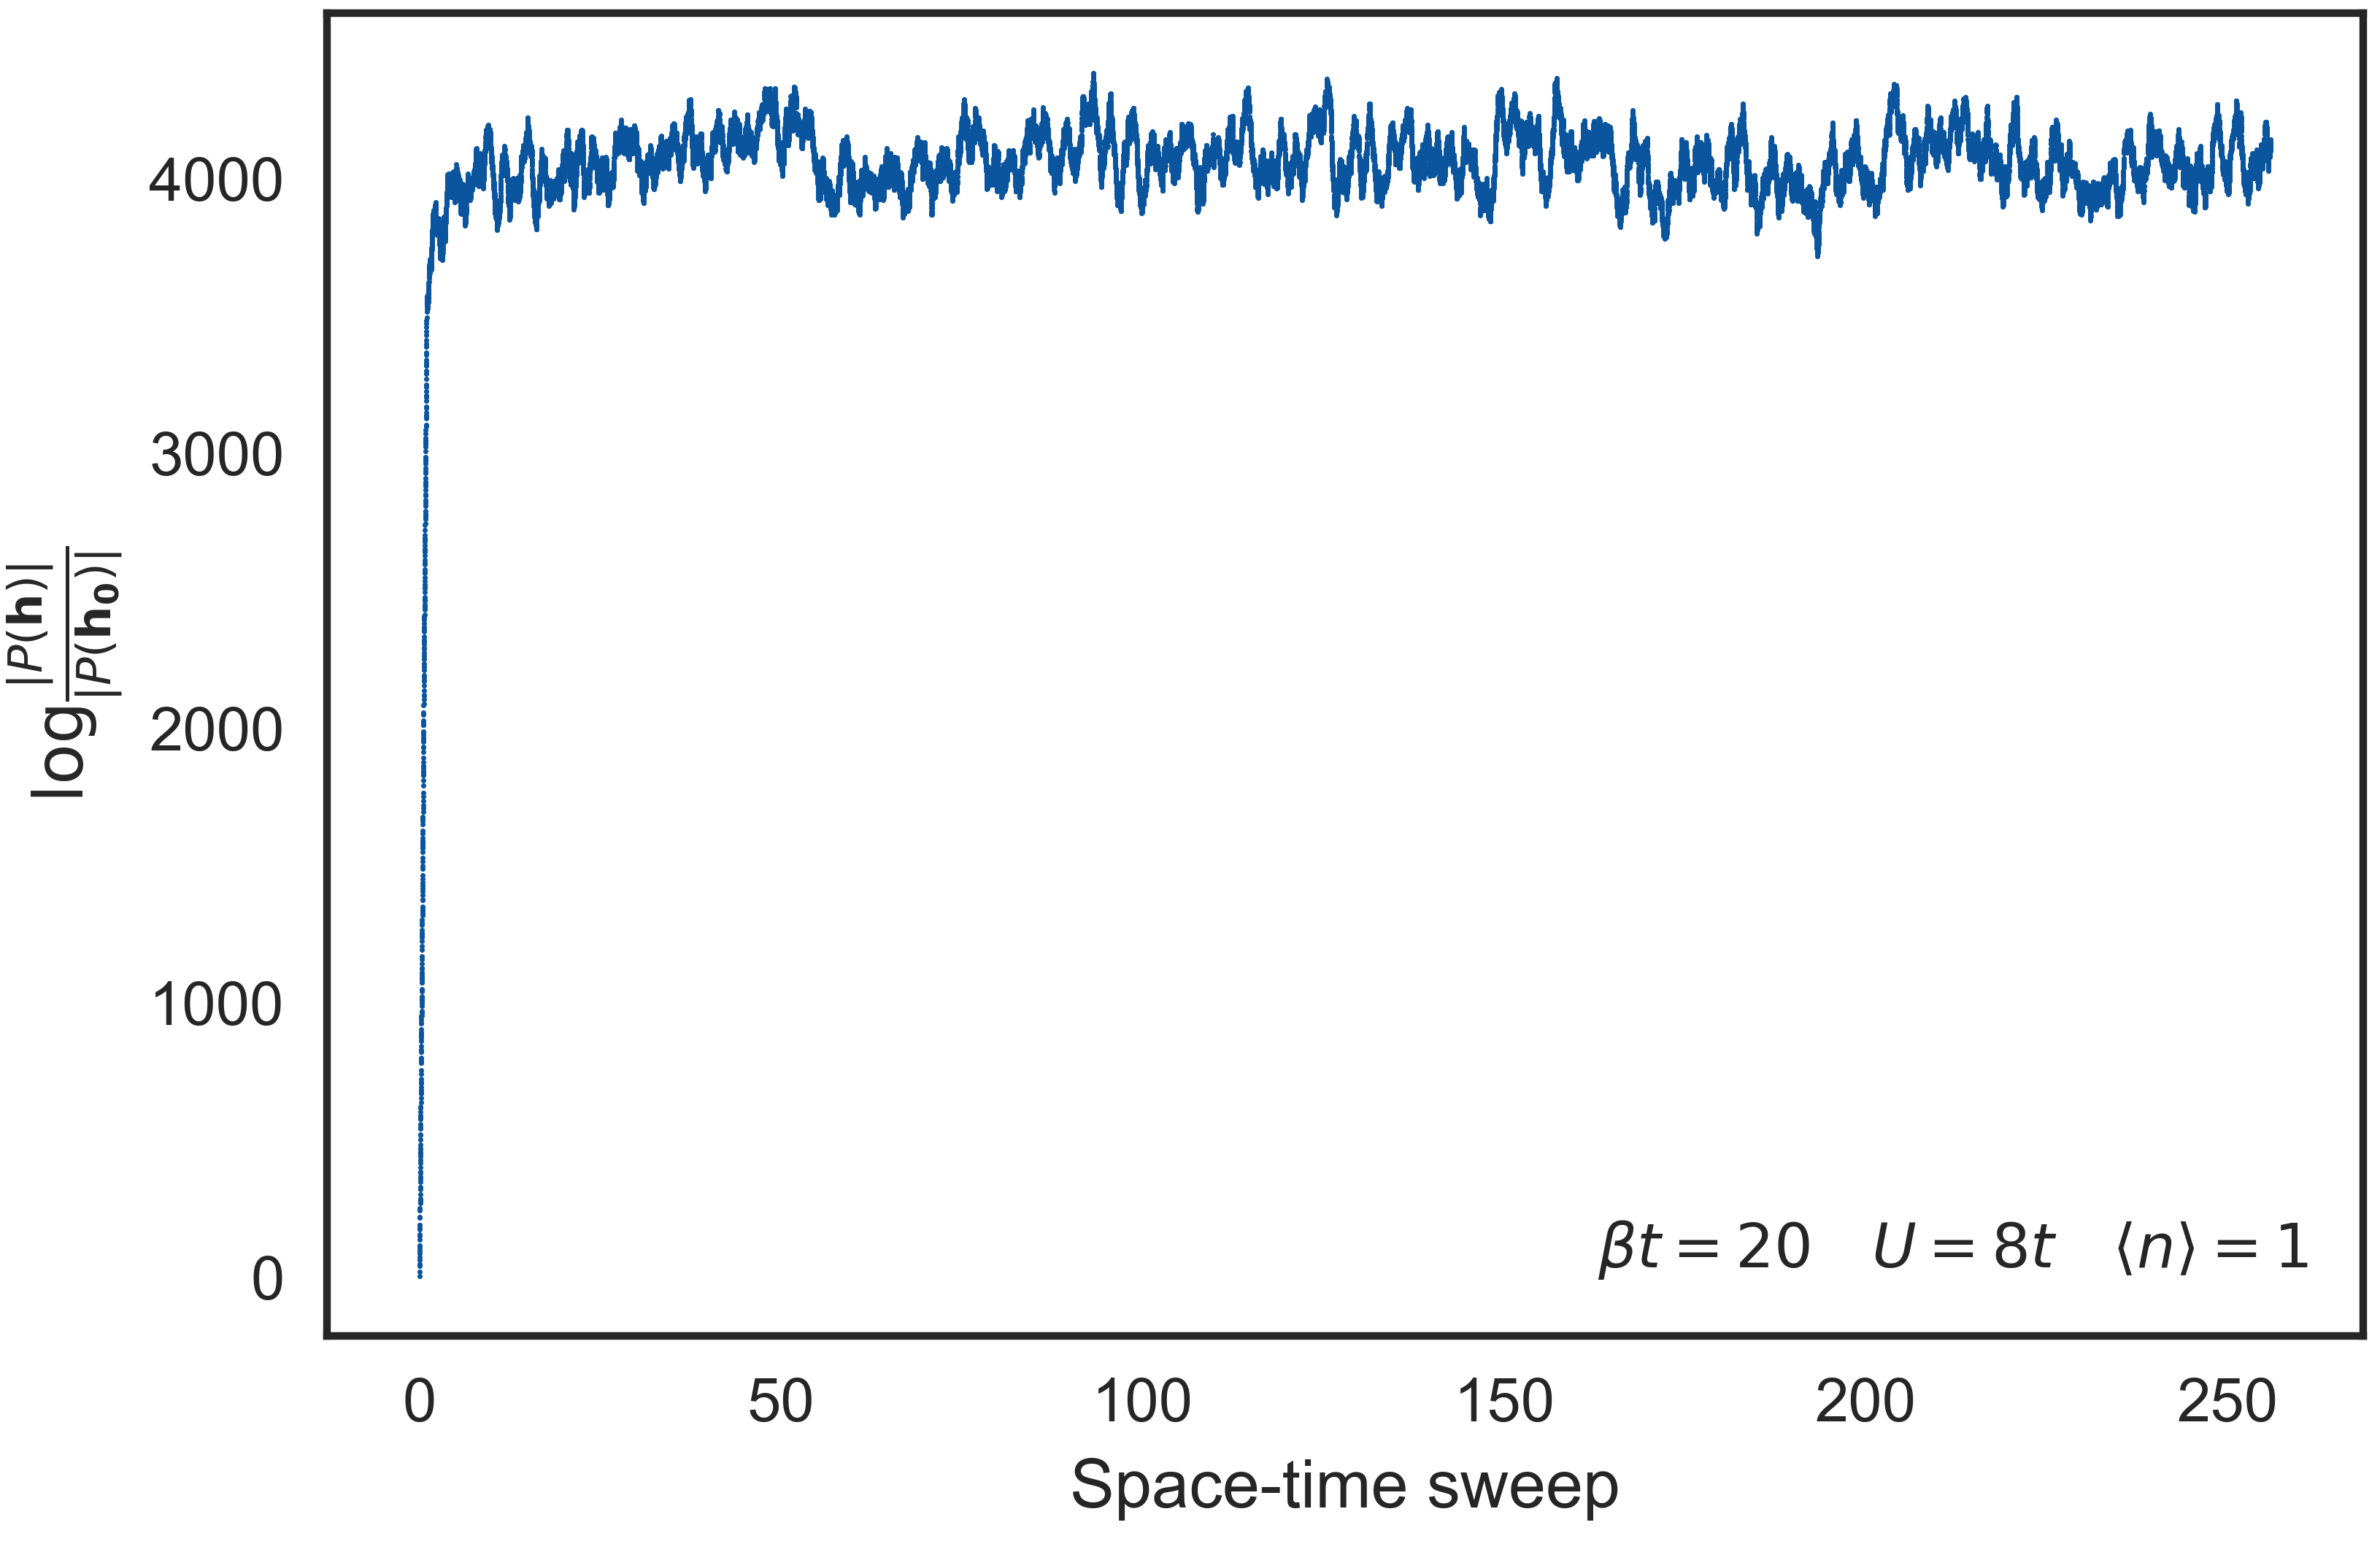
\includegraphics[scale=0.55]{Afqmc/Log-weights_N=64sites.png}
\hspace{-0.8cm}
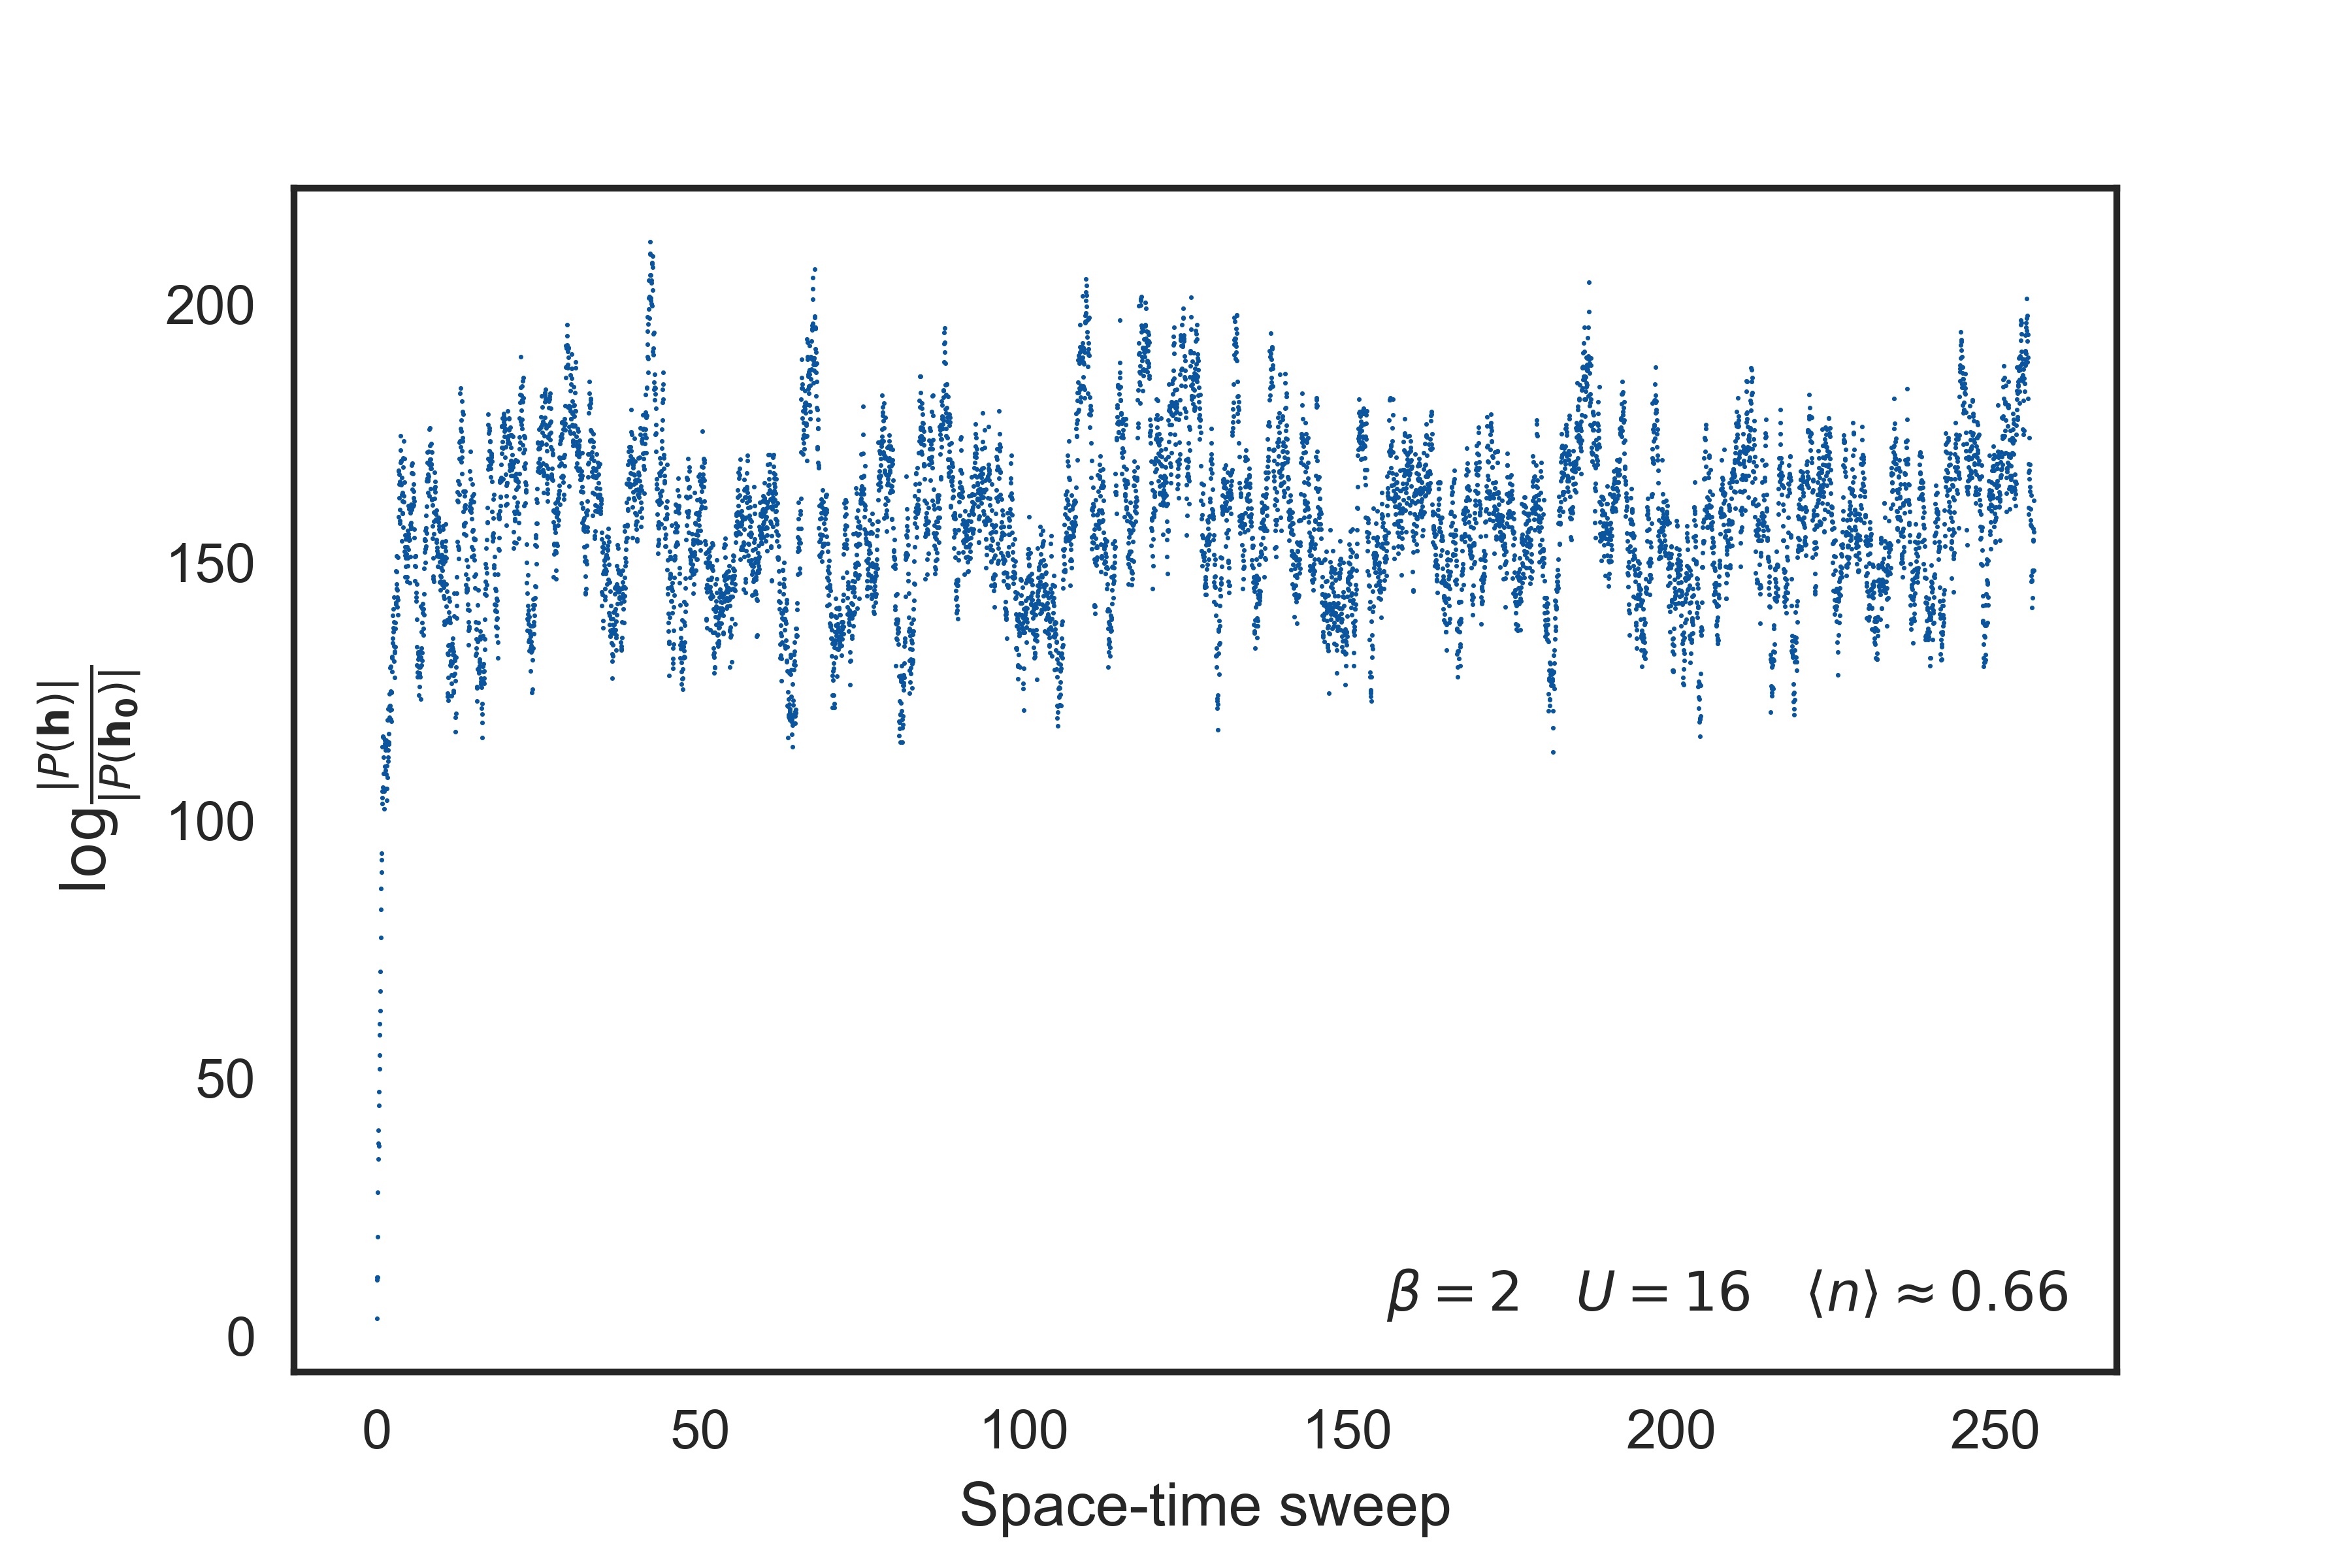
\includegraphics[scale=0.55]{Afqmc/Log-weights_N=108sites.png}
\caption[Evolution of the probability of accepted configurations.]{Evolution of the probability of accepted HS field  configurations with respect to the probability of the first randomly chosen configuration for a $8 \times 8$ square lattice and for a $9 \times 4$ $\text{Mo}\text{S}_2$ \acs{TMDNR}. Note that while we consider a higher $U$  for the \acs{TMDNR}, the statistical weights are smaller since the hoppings are normalized to $|t_0| = 0.184$, instead of being uniform and equal to one: $t= 1$, as in the square lattice. Moreover, we consider $\beta = 2$, a typical used inverse temperature, since the sign problem tends to impede accurate lower temperature simulations.}
\end{figure}
\begin{algorithm}
\caption{Auxiliary Field Quantum Monte Carlo Sampling Scheme}
\label{afqmcSampling}
\begin{algorithmic}[5]
  \STATE Initialize hoppings $\bm K$, and  HS field $\bm h$  \\
  \STATE  $(h_{l, i}) = (\pm 1)$, $ l=0,... L-1$, $i = 0, ... N-1$; $(l, i) \leftarrow (0, 0)$
  \FOR{$\text{step} = 1$ to $S$}
  \STATE \footnotesize{Propose new configuration by flipping a spin:}\normalsize{$h_{l, i}' = - h_{l, i}$} 
  \STATE \footnotesize{Compute the acceptance ratio $a_{l, i}$}:
  \normalsize{$\frac{\text{det}[\bm M_\uparrow (\bm h')]\text{det}[\bm M_\downarrow (\bm h')]}{\text{det}[\bm M_\uparrow (\bm h)]\text{det}[\bm M_\downarrow (\bm h)]}$}
  \STATE \textbf{\normalsize{Metropolis step}}
  \STATE \footnotesize{Draw random number $r \in [0,1]$}
  \IF{$r \le \min(1, a_{l, i})$}
  \STATE $\bm h = \bm h'$
  \ELSE
  \STATE $\bm h = \bm h$
  \ENDIF
  \STATE \textbf{Next space-time \say{site}}
  \IF{$i < N - 1$}
  \STATE $l = l$ , $i = i +1 $
  \ELSE
  \IF {$l < L - 1$}
  \STATE $l = l+1$ , $i = 0 $
  \ENDIF
  \IF {$l = L - 1$}
  \STATE $l = 0$ , $i=0$
  \ENDIF
  \ENDIF
  \ENDFOR
\end{algorithmic}
\end{algorithm}

The acceptance/rejection scheme leads to a rank-one update of the matrices $\bm M_\sigma (\bm h)$\footnote{We will see that it is actually more convenient to work with their inverses, the Green's matrices.}, which affords an efficient evaluation of the acceptance ratio $a_{l, i}$ \cite{hou_numerical_2009} (see appendix \ref{ap:theoAFQMC}).
The acceptance ratio is given in terms of determinants of the Green's matrices, but these need not be explicitly computed at each step.
Instead, a \emph{global} update of the Green's matrices at each step suffices to obtain the ratio between the determinants of the Green's matrices of the current and previous configurations.
This brings the computational complexity from $\mathcal{O}(N^3)$ to $\mathcal{O}(N^2)$ at each step.
This results in an overall cubic scaling of the algorithm, more precisely $\mathcal{O}(\beta N^3)$ (the process is repeated $L N$ times, and $\beta \sim L$).

Suppose we start at the first imaginary-time slice, $l = 0$.
Using the result of appendix \ref{ap:theoAFQMC}, for $i = 0$, the proposal $h_{0 0}' = - h_{0 0}$ leads to
\begin{equation}
r_{0 0} = \bigg[ 1 + \alpha_{0, \uparrow} ( 1 - \bm e_0^T \bm M_\uparrow^{-1} ( \bm h ) \bm e_0 ) \bigg] \bigg[ 1 + \alpha_{0, \downarrow} ( 1 - \bm e_0^T \bm M_\downarrow^{-1} ( \bm h ) \bm e_0 ) \bigg] \equiv d_{0, \uparrow} d_{0, \downarrow} ,
\end{equation}
where we defined the unit vectors $\bm e_0, \bm e_1, ..., \bm e_{N-1}$, and the ratios of determinants
\begin{equation*}
d_{i, \sigma} = 1 + \alpha_{i, \sigma} ( 1 - G^\sigma_{i i} ) \quad \text{with} \quad \alpha_{i, \sigma} = e^{-2 \sigma \nu h_{l i}} - 1
\end{equation*}

The most expensive operation is the computation of the $(0, 0)$ entry of $G^\sigma (\bm h)$.
However, this object is always computed in advance (it is the main object of the simulation!), so the computation of the acceptance ratio is essentially free.
Whenever a step is accepted, the Green's matrices are updated in $\mathcal{O}(N^2)$ flops, and the acceptance ratio is recomputed as our notation suggests
\begin{equation}\label{eq:updates}
\bm G^\sigma ( \bm h ) \leftarrow \bm G^\sigma ( \bm h ) - \frac{\alpha_{i, \sigma}}{r_{l, i}} \bm u_{i, \sigma} \bm w_{i, \sigma}^T \quad \quad r_{l,i} = d_{i, \uparrow} d_{i, \downarrow} ,
\end{equation}
where $\bm u_{i, \sigma} = ( \bm I - \bm G^\sigma ( \bm h ) ) \bm e_i$, and $\bm w_{i, \sigma} = [ \bm G^\sigma (\bm h) ]^T \bm e_i$.
Notice that here, $\bm G^\sigma$ is the Green's matrix at slice $l$.
If the step is accepted, the $i$-th column of the $\bm B_l ( \widetilde{\bm h_l} )$-matrix is multiplied by $e^{-2 \sigma \nu h_{l i}}$.

Only one entry of each of the Green's matrices is used at each step for sampling.
To improve the efficiency of our implementation, we can compute only the relevant entry that is required for sampling until a sweep of the space lattice is completed, at which point we need to update the entire Green's function (since this final update has complexity $\mathcal{O}(N^3)$, the complexity of the algorithm does not change, although some speed-up is expected).
This block high rank update is a  \say{delayed update} in the sense that we avoid unnecessary computations until they are absolutely needed.

This procedure generalizes for all other time slices.
First, note that the order of the operators in Eq.(\ref{eq:quadraticIdentity}) may be changed by using the cyclic property of the trace.
Concomitantly, for example, when we advance to $l = 1$, we may write the $\bm M$-matrices by wrapping the equivalent $\widehat{\bm M}$ matrices:
\begin{equation}
\bm M_\sigma ( \bm h ) = \bm B_{0, \sigma}^{-1} ( \widetilde{\bm h}_0 ) \widehat{\bm M}_\sigma (\bm h) \bm B_{0, \sigma} ( \widetilde{\bm h}_0 )  \, \quad \widehat{\bm M}_\sigma (\bm h) = \bm I + \bm B_{0, \sigma} ( \widetilde{\bm h}_0 ) \bm B_{L-1, \sigma} ( \widetilde{\bm h}_{L-1} ) \bm B_{L-2, \sigma} ( \widetilde{\bm h}_{L-2} ) ... \bm B_{1, \sigma} ( \widetilde{\bm h}_1 )
\end{equation}

The Metropolis ratio can be computed with $\widehat{\bm M}$, and the Green's functions are also wrapped :
\begin{equation}\label{eq:wrap}
r = \frac{\det[\bm M_\uparrow (\bm h')] \det[\bm M_\downarrow ( \bm h')]}{\det[\bm M_\uparrow (\bm h)] \det[\bm M_\downarrow ( \bm h)]} = \frac{\det[\widehat{\bm M}_\uparrow (\bm h')] \det[\widehat{\bm M}_\downarrow ( \bm h')]}{\det[\widehat{\bm M}_\uparrow (\bm h)] \det[\widehat{\bm M}_\downarrow ( \bm h)]} 
\quad\quad
\widehat{\bm G}^\sigma ( \widetilde{\bm h}_0) = \bm B_{0, \sigma}( \widetilde{\bm h}_0 ) {\bm G}^\sigma (\bm h) \bm B_{0, \sigma}^{-1}  ( \widetilde{\bm h}_0 )
\end{equation}

The wrapping trick makes $B_{1, \sigma} ( \widetilde{\bm h}_1)$ appear at the position of the $\widehat{\bm M}$-matrix where $\bm B_{0, \sigma} ( \widetilde{\bm h}_0)$ appeared for $l = 0$.
Thus, we can use everything that was derived for $l = 0$ with the wrapped Green's functions $\widehat{\bm G}^\sigma$.
This is repeated consecutively as we advance in imaginary-time.

Since the cost of wrapping is $\mathcal{O}(N^3)$, the cost of computing $r$ is essentially that of updating the Green's matrices.
Each update requires $2N^2$ elementary operations, so that a sweep through the HS-matrix $\bm h$ costs $2 N^3 L$ flops.
One must pay attention to the efficiency (by delayed updates), and stability of the updating and wrapping of the Green's matrices.
When numerically divergent scales are present, the instability of this scheme must be controlled by computing the Green's functions from scratch periodically.
When doing so, the stability of the product of the (potentially large) chain of $\bm B$-matrices is ensured by using QR decomposition with partial pivoting, following \texttt{QUEST}'s implementation \cite{hou_numerical_2009}.

\subsection{Checkerboard Breakup}
\label{subsec:checkerboard}

In this section, we focus on the computation of the matrix exponential $\bm B = e^{t \Delta \tau \bm K}$.
Although the cost of computing it is small, and it is done only once in the initialization phase of the algorithm, if it is done naively, the resulting matrix is dense.
This is undesired since it is multiplied repeatedly by other matrices throughout the algorithm, which has a high cost of order $\mathcal{O}(N^3)$.
Diagonalizing and exponentiating $\bm K$ results in a dense matrix of $N^2$ elements.
For uniform hoppings, we can use the \ac{FFT} and apply the exponential of the kinetic term $e^{t \Delta \tau \bm K }$ in momentum space, in which $\bm K$ is diagonal.
The drawback of this approach is two-fold: first, the system size becomes constrained to powers of 2, so that the \ac{FFT} can be applied efficiently, and, more importantly, we cannot apply it to nonuniform hoppings (which is precisely the case we are interested in in this work).
A convenient, and sparse approximation of $\bm B$ in real space is available, and it is obtained simply by applying the Trotter breakup to the exponential of the hopping:
\begin{equation}
e^{t \Delta \tau \bm K } = e^{t \Delta \tau \sum_{\left\langle i, j \right\rangle} \bm K^{(ij)} } = \prod_{\left\langle i, j \right\rangle} e^{t \Delta \tau\bm K^{(ij)}} + \mathcal{O} ( (t \Delta \tau)^2 ) ,
\end{equation}
where the sparse matrices $\bm K^{(ij)}$ have only two nonzero elements: $K_{ij}^{(ij)} = K_{ji}^{(ij)} = K_{ij}$, such that the exponential may easily be computed:
\begin{equation}
e^{t\Delta\tau \bm K^{(ij)} } = \exp \left[ t\Delta\tau
\begin{pmatrix}
1 & \dots & 0 & \dots & 0 & \dots 0 \\
\vdots & & \vdots & & \vdots & & \vdots \\
0 & \dots & \cosh (  t\Delta\tau K_{ij} ) & \dots & \sinh (  t\Delta\tau K_{ij} ) & \dots 0 \\
\vdots & & \vdots & & \vdots & & \vdots \\
0 & \dots & \sinh (  t\Delta\tau K_{ij} ) & \dots & \cosh (  t\Delta\tau K_{ij} ) & \dots 0 \\
\vdots & & \vdots & & \vdots & & \vdots \\
0 & \dots & 0 & \dots & 0 & \dots 1 \\
\end{pmatrix}
\right] ,
\end{equation}
and it is also a sparse matrix with only the $ii$, $ij$, $ji$, $jj$ elements differing from the identity.
Thus, the dense matrix multiplication involving $\bm B$ and another $N \times N$ matrix becomes a series of sparse matrix multiplications, and the complexity decreases from $\mathcal{O}(N^3)$ to $\mathcal{O}(N N_b)$, where $N_b$ is the number of bonds, a number that grows linearly with the system size for local hoppings.
For example, for the square lattice, $N_b = 2 N$.
The checkerboard breakup is particularly useful with site-dependent hoppings (indicating for example a fixed lattice distortion or a multi-orbital model), since it is both efficient and easy to implement.
Furthermore, the computation of the inverse requires only reversing the sign of the off-diagonal elements, which saves us another $\mathcal{O}(N^3)$ computation.
